\documentclass{standalone}
\usepackage{tikz}
\usetikzlibrary{patterns, positioning}


\begin{document}
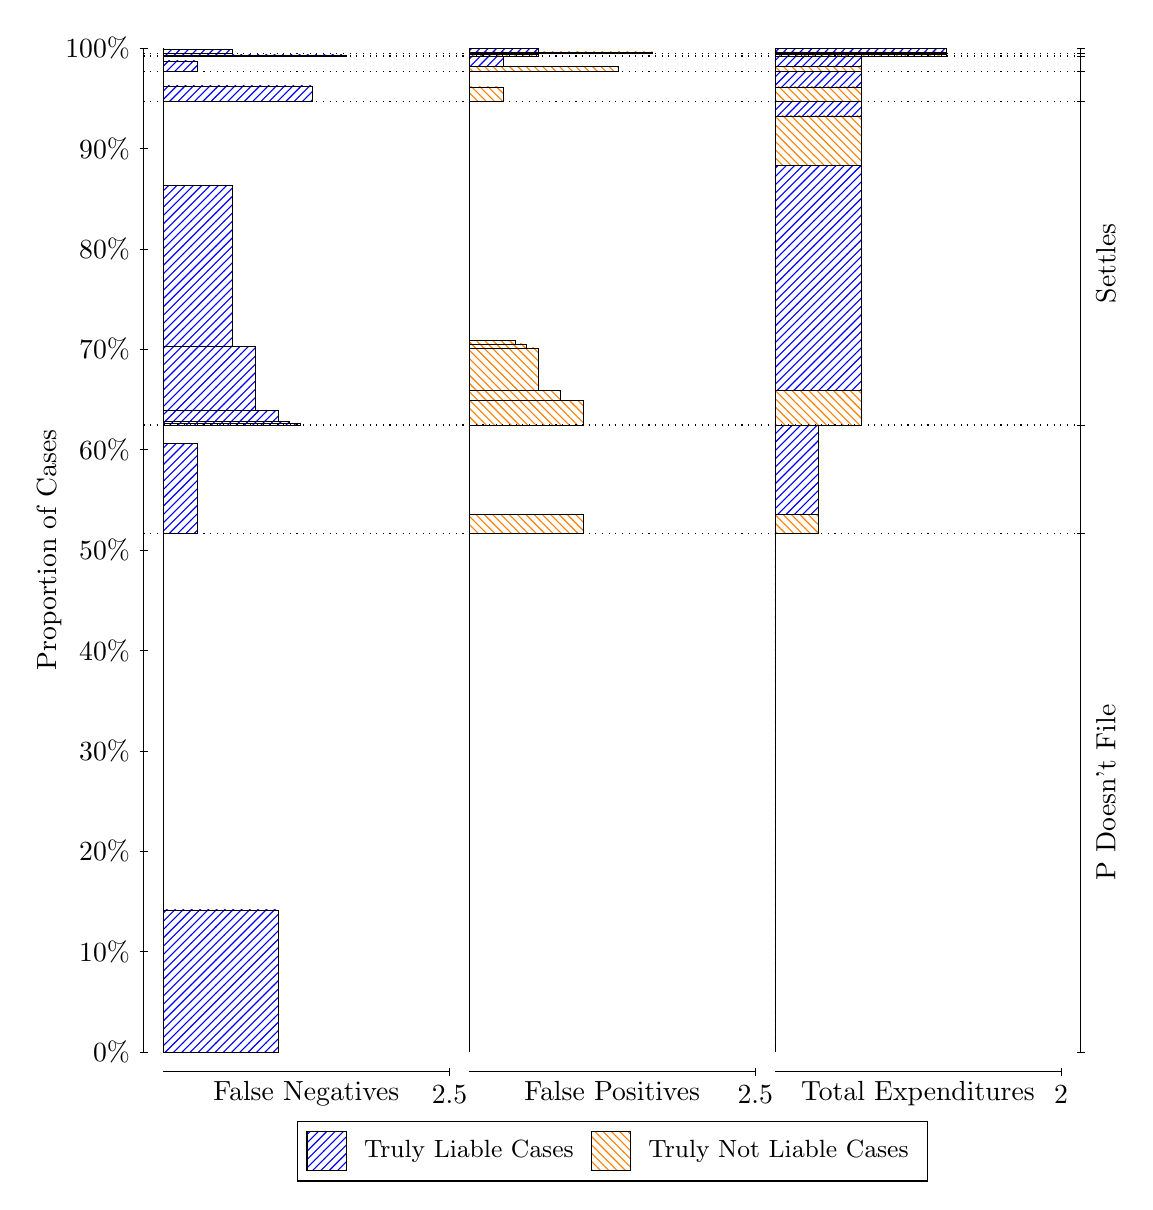
\begin{tikzpicture}
\draw[black, very thin] (1.5,1.75) -- (1.5,14.5);
\node[rotate=90, text=black, anchor=center] at (0.3, 8.125) {Proportion of Cases};
\draw[black, very thin] (1.45,1.75) -- (1.55,1.75);
\node[text=black, anchor=east] at (1.45, 1.75) {0\%};
\draw[black, very thin] (1.45,3.025) -- (1.55,3.025);
\node[text=black, anchor=east] at (1.45, 3.025) {10\%};
\draw[black, very thin] (1.45,4.3) -- (1.55,4.3);
\node[text=black, anchor=east] at (1.45, 4.3) {20\%};
\draw[black, very thin] (1.45,5.575) -- (1.55,5.575);
\node[text=black, anchor=east] at (1.45, 5.575) {30\%};
\draw[black, very thin] (1.45,6.85) -- (1.55,6.85);
\node[text=black, anchor=east] at (1.45, 6.85) {40\%};
\draw[black, very thin] (1.45,8.125) -- (1.55,8.125);
\node[text=black, anchor=east] at (1.45, 8.125) {50\%};
\draw[black, very thin] (1.45,9.4) -- (1.55,9.4);
\node[text=black, anchor=east] at (1.45, 9.4) {60\%};
\draw[black, very thin] (1.45,10.675) -- (1.55,10.675);
\node[text=black, anchor=east] at (1.45, 10.675) {70\%};
\draw[black, very thin] (1.45,11.95) -- (1.55,11.95);
\node[text=black, anchor=east] at (1.45, 11.95) {80\%};
\draw[black, very thin] (1.45,13.225) -- (1.55,13.225);
\node[text=black, anchor=east] at (1.45, 13.225) {90\%};
\draw[black, very thin] (1.45,14.5) -- (1.55,14.5);
\node[text=black, anchor=east] at (1.45, 14.5) {100\%};

\draw[black, very thin] (13.4,1.75) -- (13.4,14.5);
\draw[black, very thin] (13.35,1.75) -- (13.45,1.75);
\node[anchor=west] at (13.35, 1.75) {};
\draw[black, very thin] (13.35,8.3399) -- (13.45,8.3399);
\node[anchor=west] at (13.35, 8.3399) {};
\draw[black, very thin] (13.35,9.7119) -- (13.45,9.7119);
\node[anchor=west] at (13.35, 9.7119) {};
\draw[black, very thin] (13.35,13.824) -- (13.45,13.824);
\node[anchor=west] at (13.35, 13.824) {};
\draw[black, very thin] (13.35,14.202) -- (13.45,14.202);
\node[anchor=west] at (13.35, 14.202) {};
\draw[black, very thin] (13.35,14.399) -- (13.45,14.399);
\node[anchor=west] at (13.35, 14.399) {};
\draw[black, very thin] (13.35,14.435) -- (13.45,14.435);
\node[anchor=west] at (13.35, 14.435) {};
\draw[black, very thin] (13.35,14.5) -- (13.45,14.5);
\node[anchor=west] at (13.35, 14.5) {};

\draw[black, very thin, pattern color=blue, pattern=north east lines] (1.75,1.75) rectangle (3.2033,3.5545);
\draw[black, very thin, pattern color=orange, pattern=north west lines] (1.75,3.5545) rectangle (1.75,8.3399);
\draw[black, very thin, pattern color=blue, pattern=north east lines] (1.75,8.3399) rectangle (2.186,9.478);
\draw[black, very thin, pattern color=orange, pattern=north west lines] (1.75,9.478) rectangle (1.75,9.7119);
\draw[black, very thin, pattern color=blue, pattern=north east lines] (1.75,9.7119) rectangle (3.494,9.7299);
\draw[black, very thin, pattern color=blue, pattern=north east lines] (1.75,9.7299) rectangle (3.3487,9.759);
\draw[black, very thin, pattern color=blue, pattern=north east lines] (1.75,9.759) rectangle (3.2033,9.8991);
\draw[black, very thin, pattern color=blue, pattern=north east lines] (1.75,9.8991) rectangle (2.9127,10.714);
\draw[black, very thin, pattern color=blue, pattern=north east lines] (1.75,10.714) rectangle (2.622,12.751);
\draw[black, very thin, pattern color=orange, pattern=north west lines] (1.75,12.751) rectangle (1.75,13.824);
\draw[black, very thin, pattern color=blue, pattern=north east lines] (1.75,13.824) rectangle (3.6393,14.018);
\draw[black, very thin, pattern color=orange, pattern=north west lines] (1.75,14.018) rectangle (1.75,14.202);
\draw[black, very thin, pattern color=blue, pattern=north east lines] (1.75,14.202) rectangle (2.186,14.336);
\draw[black, very thin, pattern color=orange, pattern=north west lines] (1.75,14.336) rectangle (1.75,14.399);
\draw[black, very thin, pattern color=blue, pattern=north east lines] (1.75,14.399) rectangle (4.0753,14.414);
\draw[black, very thin, pattern color=orange, pattern=north west lines] (1.75,14.414) rectangle (1.75,14.435);
\draw[black, very thin, pattern color=blue, pattern=north east lines] (1.75,14.435) rectangle (2.622,14.484);
\draw[black, very thin, pattern color=orange, pattern=north west lines] (1.75,14.484) rectangle (1.75,14.5);
\draw[black, very thin, pattern color=orange, pattern=north west lines] (5.6333,1.75) rectangle (5.6333,6.5353);
\draw[black, very thin, pattern color=blue, pattern=north east lines] (5.6333,6.5353) rectangle (5.6333,8.3399);
\draw[black, very thin, pattern color=orange, pattern=north west lines] (5.6333,8.3399) rectangle (7.0867,8.5738);
\draw[black, very thin, pattern color=blue, pattern=north east lines] (5.6333,8.5738) rectangle (5.6333,9.7119);
\draw[black, very thin, pattern color=orange, pattern=north west lines] (5.6333,9.7119) rectangle (7.0867,10.028);
\draw[black, very thin, pattern color=orange, pattern=north west lines] (5.6333,10.028) rectangle (6.796,10.155);
\draw[black, very thin, pattern color=orange, pattern=north west lines] (5.6333,10.155) rectangle (6.5053,10.691);
\draw[black, very thin, pattern color=orange, pattern=north west lines] (5.6333,10.691) rectangle (6.36,10.744);
\draw[black, very thin, pattern color=orange, pattern=north west lines] (5.6333,10.744) rectangle (6.2147,10.785);
\draw[black, very thin, pattern color=blue, pattern=north east lines] (5.6333,10.785) rectangle (5.6333,13.824);
\draw[black, very thin, pattern color=orange, pattern=north west lines] (5.6333,13.824) rectangle (6.0693,14.007);
\draw[black, very thin, pattern color=blue, pattern=north east lines] (5.6333,14.007) rectangle (5.6333,14.202);
\draw[black, very thin, pattern color=orange, pattern=north west lines] (5.6333,14.202) rectangle (7.5227,14.265);
\draw[black, very thin, pattern color=blue, pattern=north east lines] (5.6333,14.265) rectangle (6.0693,14.399);
\draw[black, very thin, pattern color=orange, pattern=north west lines] (5.6333,14.399) rectangle (6.5053,14.42);
\draw[black, very thin, pattern color=blue, pattern=north east lines] (5.6333,14.42) rectangle (5.6333,14.435);
\draw[black, very thin, pattern color=orange, pattern=north west lines] (5.6333,14.435) rectangle (7.9587,14.451);
\draw[black, very thin, pattern color=blue, pattern=north east lines] (5.6333,14.451) rectangle (6.5053,14.5);
\draw[black, very thin, pattern color=orange, pattern=north west lines] (9.5167,1.75) rectangle (9.5167,6.5353);
\draw[black, very thin, pattern color=blue, pattern=north east lines] (9.5167,6.5353) rectangle (9.5167,8.3399);
\draw[black, very thin, pattern color=orange, pattern=north west lines] (9.5167,8.3399) rectangle (10.062,8.5738);
\draw[black, very thin, pattern color=blue, pattern=north east lines] (9.5167,8.5738) rectangle (10.062,9.7119);
\draw[black, very thin, pattern color=orange, pattern=north west lines] (9.5167,9.7119) rectangle (10.607,10.155);
\draw[black, very thin, pattern color=blue, pattern=north east lines] (9.5167,10.155) rectangle (10.607,13.007);
\draw[black, very thin, pattern color=orange, pattern=north west lines] (9.5167,13.007) rectangle (10.607,13.637);
\draw[black, very thin, pattern color=blue, pattern=north east lines] (9.5167,13.637) rectangle (10.607,13.824);
\draw[black, very thin, pattern color=orange, pattern=north west lines] (9.5167,13.824) rectangle (10.607,14.007);
\draw[black, very thin, pattern color=blue, pattern=north east lines] (9.5167,14.007) rectangle (10.607,14.202);
\draw[black, very thin, pattern color=orange, pattern=north west lines] (9.5167,14.202) rectangle (10.607,14.265);
\draw[black, very thin, pattern color=blue, pattern=north east lines] (9.5167,14.265) rectangle (10.607,14.399);
\draw[black, very thin, pattern color=orange, pattern=north west lines] (9.5167,14.399) rectangle (11.697,14.42);
\draw[black, very thin, pattern color=blue, pattern=north east lines] (9.5167,14.42) rectangle (11.697,14.435);
\draw[black, very thin, pattern color=orange, pattern=north west lines] (9.5167,14.435) rectangle (11.697,14.451);
\draw[black, very thin, pattern color=blue, pattern=north east lines] (9.5167,14.451) rectangle (11.697,14.5);
\draw[black, dotted] (1.5,8.3399) -- (13.4,8.3399);
\draw[black, dotted] (1.5,9.7119) -- (13.4,9.7119);
\draw[black, dotted] (1.5,13.824) -- (13.4,13.824);
\draw[black, dotted] (1.5,14.202) -- (13.4,14.202);
\draw[black, dotted] (1.5,14.399) -- (13.4,14.399);
\draw[black, dotted] (1.5,14.435) -- (13.4,14.435);
\draw[black, very thin] (1.75,1.5) -- (5.3833,1.5);
\node[text=black, anchor=north] at (3.5667, 1.5) {False Negatives};
\draw[black, very thin] (5.3833,1.45) -- (5.3833,1.55);
\node[text=black, anchor=north] at (5.3833, 1.45) {2.5};

\draw[black, very thin] (5.6333,1.5) -- (9.2667,1.5);
\node[text=black, anchor=north] at (7.45, 1.5) {False Positives};
\draw[black, very thin] (9.2667,1.45) -- (9.2667,1.55);
\node[text=black, anchor=north] at (9.2667, 1.45) {2.5};

\draw[black, very thin] (9.5167,1.5) -- (13.15,1.5);
\node[text=black, anchor=north] at (11.333, 1.5) {Total Expenditures};
\draw[black, very thin] (13.15,1.45) -- (13.15,1.55);
\node[text=black, anchor=north] at (13.15, 1.45) {2};

\node[text=black, centered, rotate=90] at (13.72, 5.0449) {P Doesn't File};

\node[text=black, centered, rotate=90] at (13.72, 11.768) {Settles};





\draw (7.449999999999999,1.5) node[draw=none] (baseCoordinate) {};
\begin{scope}[align=center]
        \matrix[scale=0.5, draw=black, below=0.5cm of baseCoordinate, nodes={draw}, column sep=0.1cm]{
            \node[rectangle, draw, minimum width=0.5cm, minimum height=0.5cm, pattern color=blue, pattern=north east lines] {}; &
            \node[draw=none, font=\small, text=black] (B) {Truly Liable Cases}; &
            \node[rectangle, draw, minimum width=0.5cm, minimum height=0.5cm, pattern color=orange, pattern=north west lines] {}; &
            \node[draw=none, font=\small, text=black] (B) {Truly Not Liable Cases}; \\
            };
\end{scope}

\end{tikzpicture}
\end{document}